% !TEX root = Eco-Model.tex
\section{Design of the ecosystem} % (fold)
\label{sec:design_of_the_ecosystem}
% \subsection{Preliminaries} % (fold)
% \label{sub:preliminaries}
Before introducing the design of the ecosystem, we specify some basic definitions:
\begin{compactitem}
	\item Provider: the individual who provides resource;
	\item Resource: the basic task process object with renewable capacity and unique type;
	\item Demander: the individual who publishes orders that contain bunch of tasks;
	\item Order: the task bundle like a project;
	\item Task: the basic object that needs to be processed with resource-type cooperation;
	\item Task-part: virtual resource-type segmentation unit of one task;
	\item Product: the perform result of a task;
    \item Service-call: the basic object that needs to be processed with both resource-type and resource-capacity cooperation;
    \item Job: the generalization of task and service-call;
    \item Service: the perform result of a service-call, a group of tasks;
    \item Machine: the generalization of resource and service;
	\item Platform: the place where individuals interact with others;
    \item Resource-type cooperation: resource in specific type to process a job simultaneously;
    \item Resource-capacity cooperation: part of resources in same type to process a service-call simultaneously.
\end{compactitem}

With the cloud manufacturing platform operating, demanders publish orders while providers provide resources, then they make decisions to  arrange the resources to perform tasks that decomposed from order. Most recent researchers e.g. Wu et al. \cite{Wu2013}, describe this operation procedure in cloud manufacturing as a tri-group user model that contains:\begin{inparaenum}[1)]
\item users/customers,
\item application providers and
\item physical resource providers.
\end{inparaenum}
Inspired by this model, we design the original operation mode shown in \autoref{fig:originmode} as the basis.
In this mode, individual executes activities that interact with others depicted by object flow(full lines) and information flow(dashed lines). A single order can be described by an activity-on-node(AON) network where the node represent the task and the arc the precedence relation. Each task needs to be performed with resource-type cooperation as listed in \autoref{tab:simplejobconfiguration}, and the selected resource cannot start to process the task until all of other selected resources are ready, what each resource actually processes is the task-part as show in \autoref{fig:simplejoblist}, we call the task-part is \textbf{active} when being processed, \textbf{semi-active} when selected resource is waiting as shadow in \autoref{fig:simplejoblist}, \textbf{inactive} when this part is just assigned to the job queue. Product, the performance result after the processing and assembly procedure, will be delivered to demander, then demander change the rank value of the selected resource owners according to the review of the product. 


\subsection{Nomenclature and assumptions} % (fold)
\label{ssub:assumptions_nomenclature}
\begin{table}[htbp]
  \scriptsize
\begin{tabularx}{\textwidth}{|lX|}
    \hline
    \multicolumn{2}{|l|}{\multirow{2}[0]{*}{\textbf{Nomenclature}}} \\
    \multicolumn{2}{|l|}{} \\
    $\mathcal{T}_i$ & Order that come with demander, who can be quired by $F(\cdot)$ \\
    $t_{ij}$ & Task belongs to $\mathcal{T}_i$, $t_{ij}\in\mathcal{T}_i$ \\
    $p_{ij}$ & Process duration of $t_{ij}$\\
    $\gamma_{ij}$ & Expect quality of product after the finish of $t_{ij}$\\
    $r_i$ & Release time of all $t_{ij}\in\mathcal{T}_i$\\
    $f_{ij}$ & Actual finish time of $t_{ij}$ \\
    % $f_{i}$ & Finish time of $\mathcal{T}_i$\\
    $\mathcal{P}_{ij}$ & The set of predecessor of $t_{ij}$, determined by order and some assignment procedure\\
    $mr_k$ & Resource that come with provider, who can be quired by $F(\cdot)$ \\
    $\delta_k$ & Task-part quality produced via resource $mr_k$ \\
    $C_{k,\tau}$ & Capacity of $mr_k$ at time $\tau$\\
    $A_{k,\tau}$ & Available capacity of $mr_k$ at time $\tau$\\
    $\mathcal{L}_{k,\tau}$ & The list of inactive job queue of $mr_k$ at $\tau$ with sequence\\
    $\mathcal{H}_{k,\tau}$ & The list of semi-active job of $mr_k$ at $\tau$ \\
    $\mathcal{G}_{k,\tau}$ & The set of active job of $mr_k$ at $\tau$ \\
    % $job_\theta$ & Task that need to be scheduled at $\tau_0$,  $\theta = 1,...,\abs{\mathcal{L}^{(s)}_{k,\tau_0}\cup\mathcal{G}^{(s)}_{k,\tau_0}}$\\
    $f^{(s)}_\theta$ & Ideal finish time of $job_\theta$ in $\mathcal{L}^{(s)}_{k,\tau_0}$ for schedule at $\tau_0$ . \\
    $re_j$ & Remaining process time of $t_j$ in $\mathcal{G}_{k,\tau_0}$ for schedule at $\tau_0$. \\
    % $\mathcal{A}$ & Resource type set \\
    $\mathcal{A}_{ij}$ & Resource type subset required by $t_{ij}$\\ %, $\mathcal{A}_{ij}\subset\mathcal{A}$\\
    $q_{\alpha,ij}$ & Required amount of resource with type $\alpha$ by $t_{ij}$, $\alpha\in\mathcal{A}_{ij}$\\
    $sc_l$ & Service-call generated by provider\\
    $p_l$ & Process duration of $sc_l$\\
    $r_l$ & Release time of $sc_l$\\
    $\mathcal{P}_{l}$ & The set of predecessor of $sc_{l}$\\
    $\mathcal{A}_l$ & Resource type subset required by $sc_l$ or provided by $ms_l$ \\ %, $\mathcal{A}_l\subset\mathcal{A}$\\
    $ms_l$ & Service that generated after the finish of $sc_l$\\
    $\Delta_l$ & Product quality produced via service $ms_l$\\
    $\bm{mr}_l$ & Resource member set of $ms_l$\\
    $\bm{q}_l$ & Resource member's capacity contribution set of $ms_l$\\
    $q_{\alpha,l}$ & Need resource capacity of $sc_l$ with type $\alpha$,$\alpha\in\mathcal{A}_{l}$\\
    $\bm{\alpha}_l$ & Subset of $\bm{q}_l$ that consists of all the capacities of type $\alpha$ resources in $\bm{mr}_l$\\
    $\mathcal{L}_{l,\tau}$ & The list of job queue of $ms_l$ at $\tau$ with sequence\\
    $\mathcal{G}_{l,\tau}$ & The set of active job of $ms_l$ at $\tau$ \\
    $\mathcal{R}_{ij,\tau}$ & Resource candidates set for $t_{ij}$ to select\\
    $\mathcal{B}_{ij,\tau}$ & Resource candidate types set for $t_{ij}$\\
    $\mathcal{S}_{ij,\tau}$ & Service candidates set for $t_{ij}$ to select\\
    $\mathcal{R}_{l,\tau}$ & Resource candidates set for $sc_l$ to select\\
    $\mathcal{B}_{l,\tau}$ & Resource candidate types set for $sc_l$\\
    $R(\cdot)$ & Rank inquire function about provider\\
    $F(\cdot)$ & Owner inquire function about resource or service\\
    $P(\cdot)$ & Type inquire function about resource type\\
    $\bm{x}$ & Bold font of the variable($x$) means the temp set of a bunch of these variables\\
    \hline
\end{tabularx}
\end{table}
Since demander and provider continuous arrives, there is no upper bound of the subscripts
$(i,j,k,l,\alpha)$.
To scope our research, we make some assumptions as follows for the original mode, while in other extensions, some of the assumptions will be modified.
\begin{compactitem}
\item Each single task should be assembled by its task-parts, and these parts should be processed simultaneously;
\item The quality of product is determined by the worst quality of the selected resource;
\item Resource are renewable that the available capacity will be restored when the processing procedure finished;
\item Resource quality comply normal distribution with given mean and standard deviation by provider when registered;
\item Cooperation and processing procedure cannot be interrupted;
\item Provider can only schedule task-parts in inactive status.
\end{compactitem}



% \vspace{-2.5em}
% subsubsection assumptions_nomenclature (end)
\subsection{Master plan for original and extended modes} % (fold)
\label{ssub:master_plam}
In original mode, a single \textbf{order} consists of a set $\mathcal{T}_i = \left\{ t_{i1},t_{i2},\dots\right\}$ of tasks, the tasks are interrelated by kinds of constraints. First, precedence constraints force \textbf{task} $t_{ij}$ not to be started before all its immediate predecessors $\mathcal{P}_{ij}$. Second, performing the tasks requires resources with limited capacities. Third, resources cooperation requires all the task-parts in active status.
A single \textbf{resource}($mr_k$) belongs to only one type. While being processed, task $t_{ij}$ requires $q_{\alpha,ij}$ units capacity of the resources with each type $\alpha\in\mathcal{A}_{ij}$ during every period of its non-preemptable duration $p_{ij}$. Each resource $mr_k$ has a limited capacity $C_{k,\tau}$ and available capacity $A_{k,\tau}$ at any point in time $\tau$. This plan is much like the settings in RCPSP\cite{Kolisch1999} except that the task here need to be processed with resource cooperation.

The relation of proposed extended modes is shown in \autoref{fig:modes},
\begin{figure}[htbp]
    \centering
    \resizebox{\textwidth}{!}{% !TEX root = flow_head.tex
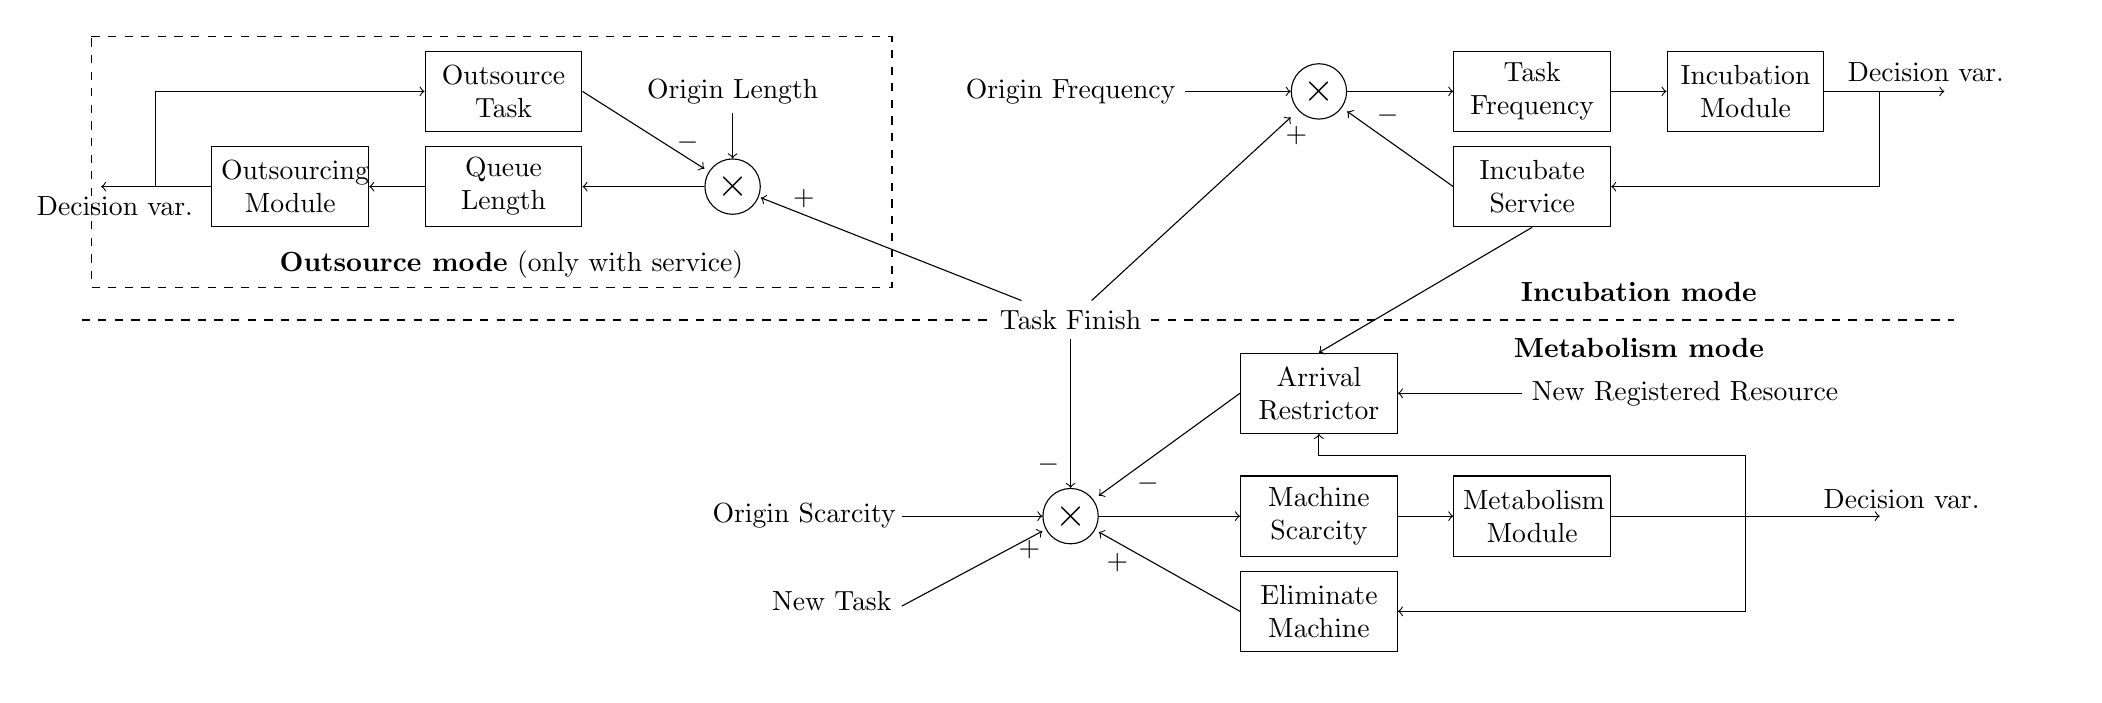
\begin{tikzpicture}[node distance=5mm and 5mm,
square/.style={
% The shape:
rectangle,
draw=black,
minimum size=2.9em,
text width=5em,
text centered
},
coord/.style={
coordinate,
% on chain,
% on grid,
% node distance=6mm and 25mm
},
circle/.style={
rectangle,minimum size=2em,rounded corners=1em,
draw=black
},
skip loop/.style={to path={-- ++(0,#1) -| (\tikztotarget)}}
]
\matrix[row sep=0.5em,column sep=2em] {
% First row:
\node (s1) [coord] {}; & & & & & \node (s2) [coord]{} ; & & & & & & \\
& & &   \node   (out) [square] {Outsource Task} ; &  \node (originl) {Origin Length} ; &  &\node (origin) {Origin Frequency} ; & \node (compare) [circle] {\Large$\times$}; &  \node (frequency) [square] {Task Frequency} ; & \node (incubate) [square] {Incubation Module} ; & \node (node) [coord] {} ; & \node (end) [coord] {}; \\
\node (end1)  {}; & \node (node1) [coord] {} ; & \node (outsource) [square] {Outsourcing Module} ; &\node (length) [square] {Queue Length} ; & \node (compare1) [circle] {\Large$\times$};  & & & & \node (sc) [square] {Incubate Service} ; & & & \\
\\
&& \node (o1){};& &\node (o2){}; \\
\node (s3) [coord]{}; &  & & & & \node (s4) [coord]{}; &  & & & & &\\
\node (tfs) {};& & \node (metam1) {};& &\node (metam2) {};& &  \node (tf) {Task Finish}; & &\node (incm1){}; & \node (incm2){};& &\node (tfe) {};\\
&&&&& & & \node (machinein) [square] {Arrival Restrictor}; & \node (add) {};  &  & &\\
&&&&&&&&&&&\\
&&&&&&&&&&&\\
& & && &\node (origin2) {};  & \node (compare2) [circle] {\Large$\times$}; &  \node (scarcity) [square] {Machine Scarcity}; & \node (metabolism) [square] {Metabolism Module}; &\node (node2) [coord] {}; &\node (end2) [coord] {};\\
&&&&&\node (task) {}; &  & \node (reduce) [square] {Eliminate Machine}; &  & & &\\
&&&&& &  &  & & & & &&  \\
};
\path (origin) edge[->] (compare) (tf) edge[->] (compare) (compare) edge[->] (frequency) (frequency) edge[->] (incubate) (incubate) edge[->] (end);
\path (sc.west) edge[->] (compare);
\draw [->] (node) |- (sc) ;
\path (tf) to node [near end,xshift=2em,yshift=1em] {$+$} (compare) (sc) to node [near end,xshift=0.5em] {$-$} (compare) (incubate) to node [yshift=0.7em,xshift = 1.5em] {Decision var.} (end);
\draw[dashed] (s1) -- (s2) -- (s4) -- (s3) -- (s1);
\draw[dashed,thick](tfs.west) -- (tf.west) (tf.east) -- (tfe.east);

\path (originl) edge[->] (compare1) (compare1) edge[->] (length) (length) edge[->] (outsource) (outsource) edge[->] (end1);
\path (out.east) edge[->] (compare1);
\draw [->] (node1) |- (out) ;
\path (out) to node [near end,xshift=0.5em,yshift=0.7em] {$-$} (compare1) (outsource) to node [near end,yshift=-0.7em,xshift = -0.5em] {Decision var.} (end1);

\draw[->] (tf) edge (compare1) (tf) edge (compare2);
\path (tf) to node [yshift=0.9em,xshift=-0.8em,near end] {$+$} (compare1) (tf) to node [xshift=-0.8em,yshift=-0.5em,near end] {$-$} (compare2);

\draw (sc.south) edge[->] (machinein.north);

\path (add) edge[->] (machinein) (machinein.west) edge[->] (compare2) (compare2) edge[->] (scarcity) (scarcity) edge[->] (metabolism);
\path (origin2) edge[->] (compare2);
% \path (tf) edge[->] (compare2);
\path (reduce.west)  edge[->] (compare2);
\draw [->] (metabolism) -- (end2) ;
\draw [->]  (task) -- (compare2);
\path (node2) edge[->,skip loop=2.2em] (machinein);
\draw [->] (node2) |- (reduce);
\path (machinein.west) to node [near end,yshift=-0.5em,xshift=0.5em] {$-$} (compare2);
% \path (tf) to node [near end,xshift=0.5em] {$-$} (compare2);
\path (task) to node [near end,xshift=0.8em] {$+$} (compare2);
\path (reduce) to node [near end,xshift=-0.6em,yshift=-0.8em] {$+$} (compare2);
\path (node2) to node [near end,xshift=2em,yshift=0.6em] {Decision var.} (end2);
\path (add) to node [near start, xshift=7em] {New Registered Resource}(machinein) (origin2) to node [near start,xshift=-4.8em]{Origin Scarcity}(compare2) (task) to node [near start,xshift=-3.8em,yshift=-0.5em]{New Task} (compare2);

\path (o1) to node {\textbf{Outsource mode} (only with service)} (o2);
\path (incm1) to node [yshift=1em]{\textbf{Incubation mode}} (incm2) (incm1) to node [yshift=-1em]{\textbf{Metabolism mode}} (incm2);
\end{tikzpicture}}
    \caption{Three Extended modes}
    \label{fig:modes}
\end{figure}
incubation and outsourcing mode are options for provider, while metabolism mode is option for platform operator, and the outsourcing mode can only be applied if incubation mode is applied because only the task that processed by service can be outsourced.

% subsubsection master_plan (end)
% subsection preliminaries (end)

\subsection{Original mode} % (fold)
\label{sub:interactions_and_decisions}
% \subsubsection{Provider respond to type-matched task}
% \label{subs:Response_for_type_matched_task}

\begin{figure}[htbp]
    \centering
    \resizebox{0.9\textwidth}{!}{% !TEX root = flow_head.tex
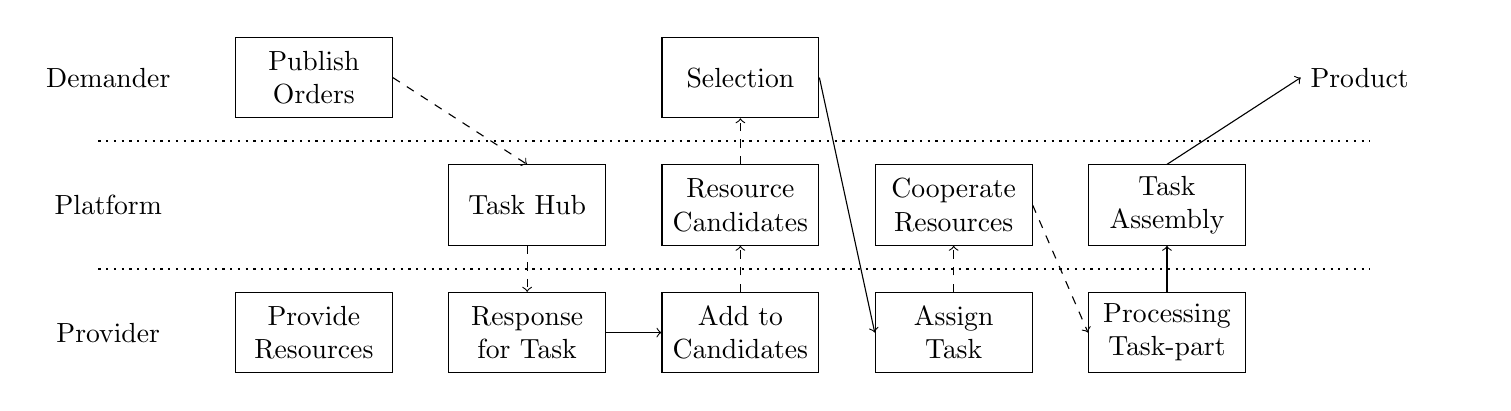
\begin{tikzpicture}[node distance=5mm and 5mm,
square/.style={
% The shape:
rectangle,
draw=black,
minimum size=2.9em,
text width=5em,
text centered
},
circle/.style={
rectangle,minimum size=1em,rounded corners=0.5em,
draw=black
}
]
\matrix[row sep=0.5em,column sep=2em] {
% First row:
\node (order) {Demander};& \node (task) [square]{Publish Orders}; &  & \node (select) [square]{Selection}; & & &  \node (finish) {Product}; \\
\node (start1) {}; & & & & & & \node (stop1) {}; \\
\node (plt) {Platform} ; & &  \node (tb) [square] {Task Hub} ; & \node (candidate) [square] {Resource Candidates} ; & \node (coop) [square] {Cooperate Resources}; & \node (combine) [square] {Task Assembly};\\
\node (start2) {}; & & & & & & \node (stop2) {}; & \\
\node (provider) {Provider};  & \node (resource) [square]{Provide Resources}; & \node (response) [square] {Response for Task}; & \node (add) [square]{Add to Candidates}; & \node (match) [square]{Assign Task}; & \node (process) [square] {Processing Task-part};  &\\
};
\draw[dotted,thick] (start1.west) -- (stop1.east) (start2.west) -- (stop2.east);
\path[->,dashed] (task.east) edge (tb.north) (tb) edge (response) (add) edge (candidate) (candidate) edge (select) (match) edge (coop) (coop.east) edge (process.west);
\path[->] (response) edge (add) (select.east) edge (match.west) (process) edge (combine) (combine.north) edge (finish.west);
% \path (order) edge[->] (task) (task) edge[->] (match) (match) edge[->] (coord) (coord) edge[->] (process) (process) edge[->] (finish) (provider) edge[->] (resource) (resource) edge[->] (match);
\end{tikzpicture}}
    \caption{Original mode}
    \label{fig:originmode}
\end{figure}

A provider makes decision at time $\tau\ge r_i$ to respond  to task if the belonging resource $mr_k$ was type-matched with $t_{ij}$ ($P(mr_k)\in\mathcal{A}_{ij}$). If $A_{k,\tau} \ge q_{\alpha,ij}$, the provider will respond to the task need, demander of $t_{ij}$ will add $mr_k$ to $\mathcal{R}_{ij,\tau}$ and $P(mr_k)$ to $\mathcal{B}_{ij,\tau}$. If $mr_k$ is finally selected, available capacity of $mr_k$ will change to $A_{k,\tau} := A_{k,\tau} - q_{\alpha,ij}$. This available capacity will be restored back to after the finish of $t_{ij}$ part.

% \subsubsection{Demander select from resource candidates}
% \label{subs:select_resource_candidates}
A demander makes decision about resource selection from $\mathcal{R}_{ij,\tau}$ when $\mathcal{B}_{ij,\tau} = \mathcal{A}_{ij}$. Without loss of generality, we suppose at time $\tau \ge r_i$, the decision-making of demander can be described as follows,
\begin{equation}
\max_{\forall \bm{k}}\left( \delta_{\bm{k}},
R\left( F\left( mr_{\bm{k}} \right) \right), \abs{\mathcal{L}_{\bm{k},\tau} }
\right) \label{eq:selectresaim}
\end{equation}
\begin{numcases}{\text{s.t.}}
q_{\alpha,ij} \le C_{k_{\alpha},\tau} & $\alpha\in\mathcal{A}_{ij}$\label{eq:rescaplimit}\\
\mathcal{R}_{\alpha,\tau} = \left\{ mr| mr\in\mathcal{R}_{ij,\tau}, P(mr) = \alpha \right\} & $\alpha\in\mathcal{A}_{ij}$\label{eq:restypeabstract}\\
\mathcal{R}_{ij,\tau} = \bigcup_{\alpha\in\mathcal{A}_{ij}}\mathcal{R}_{\alpha,\tau} & \label{eq:nrc}\\
\bm{k} = \left[k_1,\dots ,k_\alpha,\dots,k_{\abs{\mathcal{A}_{ij}}} \right] & \label{eq:decisionvectork}\\
k_\alpha \in \left\{ k | mr_k \in \mathcal{R}_{\alpha,\tau} \right\} &$\alpha\in\mathcal{A}_{ij}$ \label{eq:decisionvark}
\end{numcases}

The multi-objective in \autoref{eq:selectresaim} aims at high quality, high resource owner rank and low waiting queue length. \autoref{eq:rescaplimit} ensures that resource capacity is capable to process the task part, \autoref{eq:restypeabstract}--\ref{eq:nrc} restrict the resource candidates' type in the task configuration, \autoref{eq:decisionvectork}--\ref{eq:decisionvark} describe decision variables, the demander should make decision to select resources in each type.

% \subsubsection{Provider assign task-part in selected resource} % (fold)
% \label{subs:assign_in_select_resource}
If $mr_k$ was selected by the demander of $t_{ij}$, then the provider will add $t_{ij}$ part to $\mathcal{H}_{k,\tau}$ if $\abs{\mathcal{L}_{k,\tau}}=0,A_{k,\tau}\ge q_{\alpha,ij}$, or to  $\mathcal{L}_{k,\tau}$ otherwise.
% \begin{subnumcases}{}
% \mathcal{H}_{k,\tau} := \mathcal{H}_{k,\tau} \cup \{t_{ij}\} & if $\abs{\mathcal{L}_{k,\tau}}=0,A_{k,\tau}\ge q_{\alpha,ij}$ \label{eq:addtobuffer}\\
% \mathcal{L}_{k,\tau} := \mathcal{L}_{k,\tau} \cup \{t_{ij}\} & otherwise
% \end{subnumcases}
If all the part of $t_{ij}$ are in semi-active status, then these providers will change all the task-part status from semi-active to active and add $t_{ij}$ to $\mathcal{G}_{k,\tau}$.
% subsubsection assign_in_selected_resource (end)
% subsection interactions_and_decisions (end)

\subsection{Incubation mode} % (fold)
\label{sub:incubation_mode}
Incubation mode is one extension for the original mode, the purpose of this mode is to remove the cooperation and assembly procedure in advance by gathering types of resources with certain quota into manufacturing service, which will be incubated as shown in incubation part of \autoref{fig:modes}.
% \begin{figure}[htbp]
%     \centering
%     \resizebox{0.7\textwidth}{!}{% !TEX root = flow_head.tex
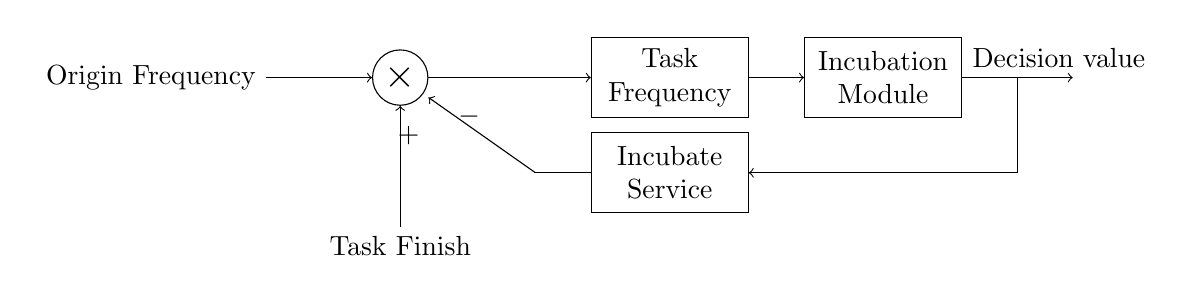
\begin{tikzpicture}[node distance=5mm and 5mm,
square/.style={
% The shape:
rectangle,
draw=black,
minimum size=2.9em,
text width=5em,
text centered
},
coord/.style={
coordinate,
% on chain,
% on grid,
% node distance=6mm and 25mm
},
circle/.style={
rectangle,minimum size=2em,rounded corners=1em,
draw=black
},
skip loop/.style={to path={-- ++(0,#1) -| (\tikztotarget)}}
]
\matrix[row sep=0.5em,column sep=2em] {
% First row:
\node (origin) {Origin Frequency} ; & \node (compare) [circle] {\Large$\times$}; & & \node (frequency) [square] {Task Frequency} ; & \node (incubate) [square] {Incubation Module} ; & \node (node) [coord] {} ; & \node (end) [coord] {}; \\
& & \node (p1) [coord] {} ; & \node	(sc) [square] {Incubate Service} ; & & & \\
& \node (tf) {Task Finish}; & & & & &\\
};
\path (origin) edge[->] (compare) (tf) edge[->] (compare) (compare) edge[->] (frequency) (frequency) edge[->] (incubate) (incubate) edge[->] (end);
\path (sc) edge (p1) (p1) edge[->] (compare);
\draw [->] (node) |- (sc) ;
\path (tf) to node [near end,xshift=0.3em] {$+$} (compare) (p1) to node [near end,xshift=0.5em] {$-$} (compare) (incubate) to node [yshift=0.7em,xshift = 1.5em] {Decision value} (end);
\end{tikzpicture}}
%     \caption{Incubation mode}
%     \label{fig:serviceincubatemode}
% \end{figure}
\begin{figure}[htbp]
    \centering
    \scriptsize
    \resizebox{.65\textwidth}{!}{% !TEX root = flow_head.tex


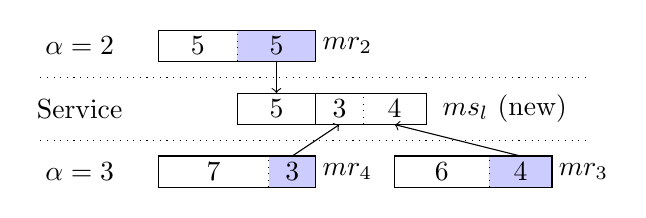
\begin{tikzpicture}
\fill[blue!20!] (10mm,0) rectangle (20mm,4mm);
\draw (0,0) rectangle (20mm,4mm) (24mm,2mm) node{$mr_2$};
\draw (5mm,2mm) node{5} (15mm,2mm) node{5} (-1cm,2mm) node{$\alpha=2$} (12mm,2mm);
\draw[dotted] (10mm,0) -- (10mm,4mm);

\draw[->] (15mm,0) edge (15mm,-4mm) (17mm,-12mm) edge (23mm,-8mm) (46mm,-12mm) edge (30mm,-8mm);
% \draw[->,xshift=30mm](41mm,-12mm) edge (20mm,-8mm);

\draw[dotted,yshift=-2mm] (-1.5cm,0) -- (5.5cm,0);

\draw[yshift=-8mm,xshift=10mm] (0,0) rectangle (24mm,4mm) (34mm,2mm) node{$ms_l$ (new)};
\draw[yshift=-8mm,xshift=10mm] (10mm,0) -- (10mm,4mm);
\draw[yshift=-8mm,dotted,xshift=10mm] (16mm,0) -- (16mm,4mm);
\draw[yshift=-8mm,xshift=10mm] (5mm,2mm) node{5} (13mm,2mm) node{3} (20mm,2mm) node{4} (-2cm,2mm) node{Service};

\draw[dotted,yshift=-10mm] (-1.5cm,0) -- (5.5cm,0);

\fill[blue!20!,yshift=-16mm] (14mm,0) rectangle (20mm,4mm);
\fill[blue!20!,yshift=-16mm,xshift=30mm](20mm,4mm) rectangle +(-8mm,-4mm);
\draw[yshift=-16mm] (0,0) rectangle (20mm,4mm) (24mm,2mm) node{$mr_4$};
\draw[yshift=-16mm,xshift=30mm] (0,0) rectangle (20mm,4mm) (24mm,2mm) node{$mr_3$};
\draw[yshift=-16mm,dotted] (14mm,0) -- +(0,4mm) ;
\draw[yshift=-16mm,dotted,xshift=30mm] (12mm,0) -- +(0,4mm);
\draw[yshift=-16mm] (7mm,2mm) node{7} (17mm,2mm) node{3} (-1cm,2mm) node{$\alpha=3$};
\draw[yshift=-16mm,xshift=30mm] (6mm,2mm) node{6} (16mm,2mm) node{4};
\end{tikzpicture}
}
    \caption{Service incubation illustration}
    \label{fig:servicefigure}
\end{figure}
After the finish of task-part, provider record the resource configuration as task frequency, when the frequency value reached some point, provider will decide to incubate such a task-specified service for the future performance. For example, if task $job_1$ in \autoref{tab:simplejobconfiguration} was finished, the first thing of incubation for the resource provider is to publish a job named \textbf{service-call} ($job_6$), which is similar to task except for the capacity dominance feature , which means capacity of selected resource will not be restored after the processing. The process result of one service-call is manufacturing \textbf{service} as shown in \autoref{fig:servicefigure}, which is actually a set of resources that may come from selected providers in the system, it's possible for more than one resources in a same type to make contributions to the incubation of one service. No more cooperation and assembly procedure are one pro of service, and product quality will no longer be restricted to the worst quality of resources for the complementary effect, while one con of service include that service can only perform specified task.
Now we can generalize task and service-call into \textbf{job}, resource and service into \textbf{machine} for the follow discuss.

% \subsubsection{Provider respond to type-matched job} % (fold)
% \label{ssub:response_in_type_matched_resource}
Apart from $mr_k$ respond to $t_{ij}$ as we explained in \autoref{subs:Response_for_type_matched_task}, there are 2 other cases in incubation mode:
\begin{asparaenum}
\item $mr_k$ respond to $sc_l$
\suspend{asparaenum}
If $mr_k$ was type-matched with $sc_l$ ($P(mr_k)\in\mathcal{A}_l$), as long as $C_{k,\tau}> 0$, provider of $mr_k$ will respond to the service-call. If $mr_k$ was finally selected, both available capacity and capacity will change as \autoref{eq:capq}--\ref{eq:cap0}, and these capacity will not be restored even after the finish of $sc_l$ part. Provider of $sc_l$ will add $mr_k$ to $\mathcal{R}_{l,\tau}$ and $P(mr_k)$ to $\mathcal{B}_{l,\tau}$.
\resume{asparaenum}
\item $ms_l$ respond to $t_{ij}$
\end{asparaenum}
Service is task-oriented machine, so if type-matched ($\mathcal{A}_{ij} =\mathcal{A}_l,\sum_{q\in\bm{\alpha}_l} q = q_{\alpha,ij}$), provider of it will respond to $t_{ij}$ as soon as possible, demander will add $ms_l$ to $\mathcal{S}_{ij,\tau}$.

% subsubsection response_in_type_matched_resource (end)

% \subsubsection{Demander select from machine candidates} % (fold)
% \label{ssub:selection_in_resource_candidates_for_service_call}
Apart from demander of $t_{ij}$ select $mr_k$ as we explained in \autoref{subs:select_resource_candidates} that $\mathcal{B}_{ij,\tau} = \mathcal{A}_{ij},\abs{\mathcal{S}_{ij,\tau}}=0$, there are 3 other cases in incubation mode:

\begin{asparaenum}
\item Select $mr_k$ for $sc_l$ when $\mathcal{B}_{l,\tau} = \mathcal{A}_l$
\suspend{asparaenum}
Provider of $sc_l$ select resource from $\mathcal{R}_{l,\tau}$ is similar to \autoref{eq:selectresaim}--\ref{eq:decisionvark}, but the difference is that the $\bm{l}_{\alpha}$ here is also a set of selected resources with type $\alpha$, $\bm{l}_{\alpha}$ is subset of decision variable $\bm{l}$. Selected resources capacity will change as \autoref{eq:capq}--\ref{eq:cap0}, and if the sum of capacity quantity in $\bm{l}_{\alpha}$ less than the $sc_l$ required, this selection will not to be executed.
\begin{subnumcases}{}
C_{k,\tau} := C_{k,\tau} - q_{\alpha,l}& If $C_{k,\tau} \ge q_{\alpha,l}$\label{eq:capq}\\
C_{k,\tau} := 0 & otherwise \label{eq:cap0}
\end{subnumcases}



\resume{asparaenum}
\item Select $ms_l$ for $t_{ij}$ when $\mathcal{B}_{ij,\tau}\subset\mathcal{A}_{ij},|\mathcal{S}_{ij,\tau}|>0$
\suspend{asparaenum}
This situation implies that the resource candidates are not enough and there exists service candidates.
\begin{equation}
\max_{\forall l}\left( \Delta_{l}, R\left(F\left(ms_{l}\right)\right), \abs{\mathcal{L}_{l,\tau}}\right)\label{eq:selectserviceaim}
\end{equation}
\begin{numcases}{\text{s.t.}}
\Delta_l \sim \mathcal{N} \left(\mu_l,\sigma_l^2\right) & \label{eq:servicecomplydist}\\
\mu_l = mean\left( \bm{mr}_l , \bm{q}_l \right) & \\
\sigma_l = std\left( \bm{mr}_l , \bm{q}_l \right) & \label{eq:servicecomplydistend}\\
l \in \left\{l' |  ms_{l'} \in \mathcal{S}_{ij,\tau} \right\}  & \label{eq:decisionvariablel}
\end{numcases}

Similar to \autoref{eq:selectresaim}, \autoref{eq:selectserviceaim} is also a multi-objective function that aims at high quality, high service owner rank and low job queue length. \autoref{eq:servicecomplydist}--\ref{eq:servicecomplydistend} explain the service quality distribution parameters, \autoref{eq:decisionvariablel} is the decision variable to select one service in $\mathcal{S}_{ij,\tau}$.

\resume{asparaenum}
\item Select machine for $t_{ij}$ when $\mathcal{B}_{ij,\tau} = \mathcal{A}_{ij},\abs{\mathcal{S}_{ij,\tau}}>0$.
\end{asparaenum}
In this situation, demander of $t_{ij}$ will select ether a bunch of resources with cooperation or one single service, so the key idea here is to pre-select optimal resources and optimal service, then to compare these two optimal options to select the better one.
\begin{equation}
\max_{m\in\{l^*,\bm{k}^*\}} \left( \Delta_m,
Rank_m, \mathcal{L}_m \right) \\ \label{eq:combaim}
% \text{s.t.}\notag
\end{equation}
\begin{numcases}{\text{s.t.}}
% q_{\alpha,ij} \le C_{k_{\alpha},\tau} & \footnotesize$\alpha\in\mathcal{A}_{ij}$\\
% R_{\alpha,\tau} = \left\{ mr| mr\in\mathcal{R}_{ij,\tau}, P(mr) = \alpha \right\} & \footnotesize$\alpha\in\mathcal{A}_{ij}$\\
% \mathcal{R}_{ij,\tau} = \bigcup_{\alpha\in\mathcal{A}_{ij}}\mathcal{R}_{\alpha,\tau} & \\
% \bm{k} = \left[k_1,\dots ,k_\alpha,\dots,k_{\abs{\mathcal{A}_{ij}}} \right]& \\
% k_\alpha \in \left\{ k | mr_k \in \mathcal{R}_{\alpha,\tau} \right\} &\footnotesize$\alpha\in\mathcal{A}_{ij}$ \\
\bm{k}^* = \arg\left(\max_{\forall \bm{k}}\left( \delta_{\bm{k}},
R\left( F\left( mr_{\bm{k}} \right) \right), \abs{\mathcal{L}_{\bm{k},\tau} }
\right)\right) & \label{eq:optk}\\
Rank_{\bm{k}^*} = \min_{k\in\bm{k}^*} \left\{ R\left( F\left( mr_k \right) \right) \right\} & \label{eq:temprank}\\
\mathcal{L}_{\bm{k}^*} = \max_{k\in\bm{k}^*}\left\{ \abs{\mathcal{L}_{k,\tau}} \right\} & \label{eq:templength}\\
\Delta_{\bm{k}^*} \sim \mathcal{N} \left(\mu_{\bm{k}^*},\sigma_{\bm{k}^*}^2\right) & \label{eq:tempqualitystart}\\
\mu_{\bm{k}^*} = mean\left( \bm{mr}_{\bm{k}^*} , \bm{q}_{\bm{k}^*} \right) & \\
\sigma_{\bm{k}^*} = std\left( \bm{mr}_{\bm{k}^*} , \bm{q}_{\bm{k}^*} \right) & \\
\bm{mr}_{\bm{k}^*} = \bigcup_{k\in\bm{k}^*}mr_k  &\\
\bm{q}_{\bm{k}^*}  =\bigcup_{\alpha\in\mathcal{A}_{ij}}q_{\alpha,ij} & \label{eq:tempqualityend}\\
% \Delta_l \sim \mathcal{N} \left(\mu_l,\sigma_l^2\right) & \\
% \mu_l = mean\left( \bm{mr}_l , \bm{q}_l \right) & \\
% \sigma_l = std\left( \bm{mr}_l , \bm{q}_l \right) & \\
% l \in \left\{l' |  ms_{l'} \in \mathcal{S}_{ij,\tau} \right\}  & \\
l^* = \arg\left( \max_{\forall l}\left(\Delta_{l}, R\left(F\left(ms_{l}\right)\right), \abs{\mathcal{L}_{l,\tau}}\right)  \right) & \label{eq:optl}\\
Rank_{l^*} = R\left( F\left( ms_{l^*} \right) \right) & \\
\mathcal{L}_{l^*} = \abs{\mathcal{L}_{l^*,\tau}} & \\
m \in \left\{ l^*,\bm{k}^* \right\} \label{eq:newdicisionvariable}
\end{numcases}

Similar to other situations, \autoref{eq:combaim} is a multi-objective function that aims at high quality, high rank and low waiting queue length. \autoref{eq:optk} and \autoref{eq:optl} are the optimal decision in independent conditions, \autoref{eq:temprank}, \autoref{eq:templength} and \autoref{eq:tempqualitystart} are the virtual rank value, virtual queue length and virtual quality value that are set in the worst cases.\autoref{eq:tempqualitystart}--\ref{eq:tempqualityend} are the virtual quality value calculation procedure. \autoref{eq:newdicisionvariable} is the decision to choose one of these two partial optimal decision.

% subsubsection selection_in_resource_candidates_for_service_call (end)

% \subsubsection{Provider assign task to selected machine} % (fold)
Apart from $mr_k$ assign $t_{ij}$ when selected as we explained in \autoref{subs:assign_in_select_resource}, there are 2 other cases in incubation mode:

\begin{asparaenum}
\item Assign $sc_l$ to $mr_k$
\suspend{asparaenum}
If $mr_k$ is selected by provider of $sc_l$ at time $\tau$, the assign condition is more restrict than that in \autoref{subs:assign_in_select_resource}, it should be changed into $\abs{\mathcal{L}_{k,\tau}} = \abs{\mathcal{G}_{k,\tau}} = \abs{\mathcal{H}_{k,\tau}} = 0$, for the capacity dominance feature of service-call, we need to assign this type of job one by one. Then, the provider of $mr_k$ should change the predecessor set:
\begin{equation}
	\mathcal{P}_l := \mathcal{P}_l\cup \mathcal{L}_{k,\tau} \cup \mathcal{H}_{k,\tau}
\end{equation}
and all the task assign after $\tau$, we say $\tau'>\tau$ will set:
\begin{equation}
	\mathcal{P}_{ij} := \mathcal{P}_{ij}\cup \left\{ sc| sc\in\mathcal{L}_{k,\tau'},sc \text{ is service-call} \right\} \cup \mathcal{H}_{k,\tau'}
\end{equation}
And $A_{k,\tau}$ will be changed with the same amount in \autoref{eq:capq}--\ref{eq:cap0}.
\resume{asparaenum}
\item Assign $t_{ij}$ to $ms_l$
\end{asparaenum}
Assign $t_{ij}$ to $ms_l$ is very simple and there will be no semi-active status for $t_{ij}$, hence it will add to $\mathcal{G}_{k,\tau}$ if $\abs{\mathcal{G}_{k,\tau}}=0$, or to $\mathcal{L}_{k,\tau}$ otherwise.
% \begin{subnumcases}{}
% \mathcal{G}_{k,\tau} := \mathcal{G}_{k,\tau} \cup \{sc_{l}\} & if $\abs{\mathcal{G}_{k,\tau}}=0$ \\
% \mathcal{L}_{k,\tau} := \mathcal{L}_{k,\tau} \cup \{sc_{l}\} & otherwise
% \end{subnumcases}

% subsubsection assign_in_selected_machine (end)
% subsection operation_mode (end)




\subsection{Outsourcing mode} % (fold)
\label{sub:outsource_mode}
Outsourcing mode is one extension on the original mode and will be active when incubation mode is on that only service can perform this procedure. As shown in \autoref{fig:outsourcemode},
% \begin{figure}[htbp]
%     \centering
%     \resizebox{0.7\textwidth}{!}{% !TEX root = flow_head.tex
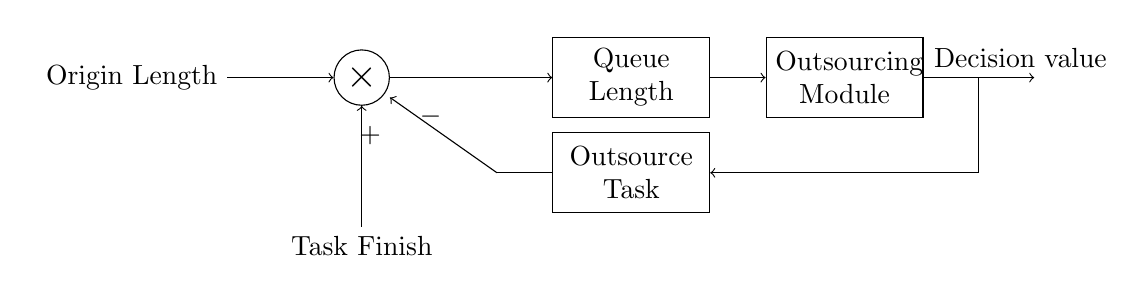
\begin{tikzpicture}[node distance=5mm and 5mm,
square/.style={
% The shape:
rectangle,
draw=black,
minimum size=2.9em,
text width=5em,
text centered
},
coord/.style={
coordinate,
% on chain,
% on grid,
% node distance=6mm and 25mm
},
circle/.style={
rectangle,minimum size=2em,rounded corners=1em,
draw=black
},
skip loop/.style={to path={-- ++(0,#1) -| (\tikztotarget)}}
]
\matrix[row sep=0.5em,column sep=2em] {
% First row:
\node (origin) {Origin Length} ; & \node (compare) [circle] {\Large$\times$}; & & \node (length) [square] {Queue Length} ; & \node (outsource) [square] {Outsourcing Module} ; & \node (node) [coord] {} ; & \node (end) [coord] {}; \\
& & \node (p1) [coord] {} ; & \node	(out) [square] {Outsource Task} ; & & & \\
& \node (tf) {Task Finish}; & & & & &\\
};
\path (origin) edge[->] (compare) (tf) edge[->] (compare) (compare) edge[->] (length) (length) edge[->] (outsource) (outsource) edge[->] (end);
\path (out) edge (p1) (p1) edge[->] (compare);
\draw [->] (node) |- (out) ;
\path (tf) to node [near end,xshift=0.3em] {$+$} (compare) (p1) to node [near end,xshift=0.5em] {$-$} (compare) (outsource) to node [yshift=0.7em,xshift = 1.5em] {Decision value} (end);
\end{tikzpicture}}
%     \caption{Outsourcing mode}
%     \label{fig:outsourcemode}
% \end{figure}
the idea of outsourcing for service is to republish active or inactive task to platform again in order to reduce its job queue length to enhance the probability to be selected by new tasks. For each single task $t_j\in\mathcal{L}_{l,\tau}\cup\mathcal{G}_{l,\tau}$, the only condition to make the outsource decision is that if the maximum delay($f_j-p_j-r_j$) of task in both status decreases. This decision highly depends on the estimation of other resources and services' performance status. Outsourcing mode makes it possible to paralleled process one job.
% subsection outsource_mode (end)

\subsection{Metabolism mode} % (fold)
\label{sub:metabolism mode}
Metabolism mode is one extension on the original mode for platform operator to control the number of individual in the system by both restrict the arrival and eliminate the current members. As shown in \autoref{fig:metabolismmode},
% \begin{figure}[htbp]
%     \centering
%     \resizebox{0.85\textwidth}{!}{% !TEX root = flow_head.tex
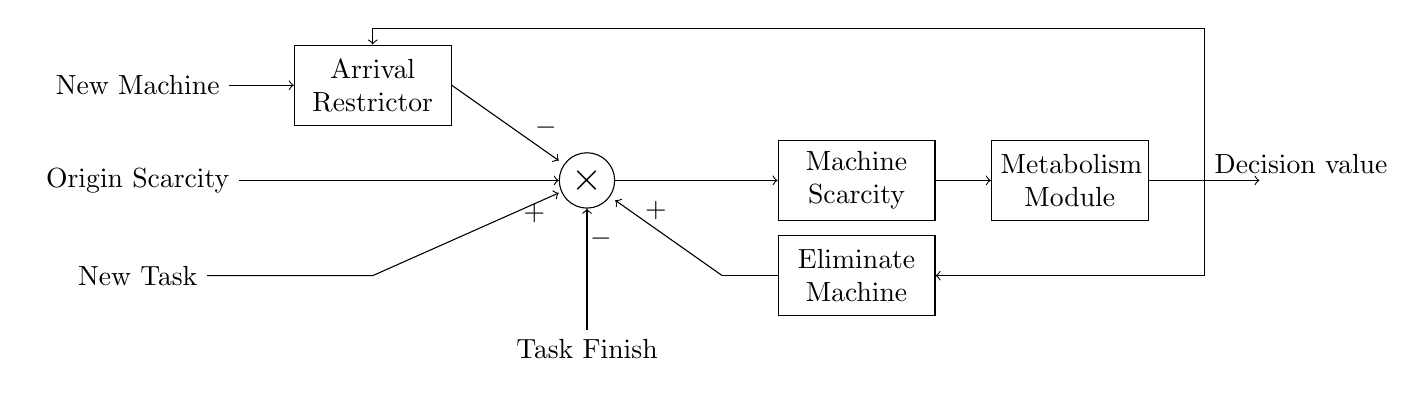
\begin{tikzpicture}[node distance=5mm and 5mm,
square/.style={
% The shape:
rectangle,
draw=black,
minimum size=2.9em,
text width=5em,
text centered
},
coord/.style={
coordinate,
% on chain,
% on grid,
% node distance=6mm and 25mm
},
circle/.style={
rectangle,minimum size=2em,rounded corners=1em,
draw=black
},
skip loop/.style={to path={-- ++(0,#1) -| (\tikztotarget)}}
]
\matrix[row sep=0.5em,column sep=2em] {
% First row:
\node (add) {New Machine}; & \node (machinein) [square] {Arrival Restrictor}; & & & & & & &\\
\node (origin) {Origin Scarcity}; & & \node (compare) [circle] {\Large$\times$}; & & \node (scarcity) [square] {Machine Scarcity}; & \node (metabolism) [square] {Metabolism Module}; &\node (node) [coord] {}; &\node (end) [coord] {};\\
\node (task) {New Task}; & \node (p1) [coord] {};& & \node (p2) [coord] {}; & \node (reduce) [square] {Eliminate Machine}; & & & & \\
& & \node (tf) {Task Finish}; &  & & & & &\\
};
\path (add) edge[->] (machinein) (machinein.east) edge[->] (compare) (compare) edge[->] (scarcity) (scarcity) edge[->] (metabolism);
\path (origin) edge[->] (compare);
\path (tf) edge[->] (compare);
\path (reduce) edge (p2) (p2) edge[->] (compare);
\draw [->] (metabolism) -- (end) ;
\draw [->]  (task) -- (p1) -- (compare);
\path (node) edge[->,skip loop=5.5em] (machinein);
\draw [->] (node) |- (reduce);
\path (machinein.east) to node [near end,yshift=0.5em,xshift=0.5em] {$-$} (compare);
\path (tf) to node [near end,xshift=0.5em] {$-$} (compare);
\path (p1) to node [near end,xshift=0.8em] {$+$} (compare);
\path (p2) to node [near end,xshift=0.5em,yshift=0.3em] {$+$} (compare);
\path (node) to node [near end,xshift=2em,yshift=0.6em] {Decision value} (end);
\end{tikzpicture}}
%     \caption{Metabolism mode}
%     \label{fig:metabolismmode}
% \end{figure}
we can define machine scarcity as $\sum_jq_{\alpha,ij} - \sum_kC_{k,\tau}$.

Platform restrict the arrival of new machine by block the registration, eliminate the current machine by their quality and owner's rank.

% Rank value is initialized to $0$ and will be changed by demander's review after the finish of task:
% \begin{subnumcases}{}
% rank := rank +
% \frac{\left( p_{ij}\cdot q_{ij} \right) \left( \delta_{ij}-\gamma_{ij} \right)}{e^{\left(f_{ij} - p_{ij} -r_{ij}\right)}} & $k\in\bm{k}$\\
% \delta_{ij} = \min_{k\in\bm{k}}\left\{ \delta_k \right\} & \\
% \delta_k \sim \mathcal{N}\left(\mu_k,\sigma_k^2 \right) & $k\in\bm{k}$
% \end{subnumcases}
% The change of rank value can be determined by:
% \begin{equation}
% 	rank := rank + \frac{ \left(\sum_{q\in\bm{q}_l}p_{ij}\cdot q \right)\left( \Delta_l -\gamma_{ij}\right) }{ e^{\left( f_{ij} - p_{ji} -r_{ij} \right)} }
% \end{equation}

% subsection controlling_rules (end)


\subsection{Provider schedule the jobs in machine} % (fold)
\label{sub:schedule_the_jobs_in_machine}
In order to reduce the idle rate, provider will schedule the inactive jobs on their machines. Since the schedule in service is a single machine scheduling problem that not on  what we focus in this study, we only discuss the job scheduling in resource. Since the  resource capacity dominance feature of service-call, it's necessary to suspend service-call in inactive status until all the job before it in $\mathcal{L}_{k,\tau}$ are finished, at the meantime, all the job after service-call should be stay in inactive status until the service-call is finished, as shown in \autoref{fig:simplejoblist}, service-call likes partition plate in $\mathcal{L}_{k,\tau}$.
\begin{figure}[htbp]
	\centering
    \large
	\resizebox{.7\textwidth}{!}{% !TEX root = flow_head.tex
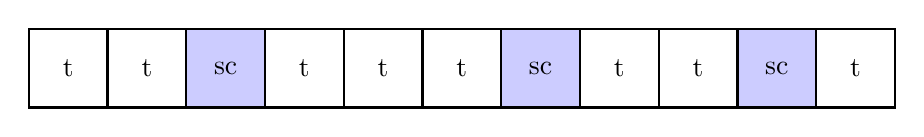
\begin{tikzpicture}

\foreach \x in {2,6,9}
	\fill[blue!20!] (\x cm, 0) rectangle +(1cm, 1cm);
\foreach \x in {2,6,9}
	\draw[xshift=.5cm] (\x cm,0.5cm) node{sc};	
\foreach \x in {0,...,10}
	\draw [thick] (\x cm, 0) rectangle +(1cm, 1cm);
\foreach \x in {0,1,3,4,5,7,8,10}
	\draw[xshift=0.5cm] (\x cm, 0.5cm) node{t};

\end{tikzpicture}
}
	\caption{Simple illustration for one $\mathcal{L}_{k,\tau}$}
	\label{fig:simplejoblist}
\end{figure}
Therefore, provider can only makes decision on the schedule of tasks before the first service-call in $\mathcal{L}_{k,\tau}$ when one of the active job in $\mathcal{G}_{k,\tau}$ was finished at $\tau_0$, we denote the set of these inactive task to be scheduled as $\mathcal{L}^{(s)}_{k,\tau_0}$.

\begin{table}[htbp]
  \centering
  \scriptsize
  \caption{Simple job configuration}
    \begin{tabular}{ccccccc}
    \toprule
    % \multicolumn{1}{c}{\multirow{2}[0]{*}{ Job}} & \multicolumn{3}{c}{Need Resource Capacity} & \multicolumn{1}{c}{\multirow{2}[0]{*}{Release Time}} & \multicolumn{1}{c}{\multirow{2}[0]{*}{Process Duration}} \\
    % \multicolumn{1}{c}{} & $Type 1$ & $Type 2$ & $Type 3$ & \multicolumn{1}{c}{} & \multicolumn{1}{c}{} \\
    Job ($\theta$) & Entity class& $q_{1,\theta}$ & $q_{2,\theta}$ & $q_{3,\theta}$ & $r_\theta$ & $p_\theta$ \\
    \midrule
    $job_1$ & task& 0     & 5     & 7     & 0     & 7 \\
    $job_2$ & task& 7     & 5     & 5     & 4     & 5 \\
    $job_3$ & task& 6     & 0     & 5     & 2     & 3 \\
    $job_4$ & task& 9	 & 4  & 6 & 1 &2 \\
    $job_5$ & task& 1 & 0 & 3 & 2 & 3\\
    $job_6$ & service-call& 1     & 0     & 3    & 0     & 1 \\
    $job_7$ & service-call& 0     & 5     & 7     & 7     & 1 \\
    \bottomrule
    \end{tabular}%
  \label{tab:simplejobconfiguration}%
\end{table}%

Specifically, a simple instance with configuration \autoref{tab:simplejobconfiguration} and schedule chart \autoref{fig:scheduleChart} will elucidate the settings.
Since the task may come from different orders, we here use the single uniform denotation $job_\theta$ to distinguish these tasks and their related variables. In this instance, as shown in \autoref{fig:simplejoblist}, horizontal dotted line constrained the available capacity of the resource for the subsequent jobs. Each finish of service-call will make the horizontal dotted line lower and it will never get higher again unless the related service is repealed.


\begin{figure}[htbp]
	\centering
	\large
	\resizebox{.8\textwidth}{!}{% !TEX root = flow_head.tex


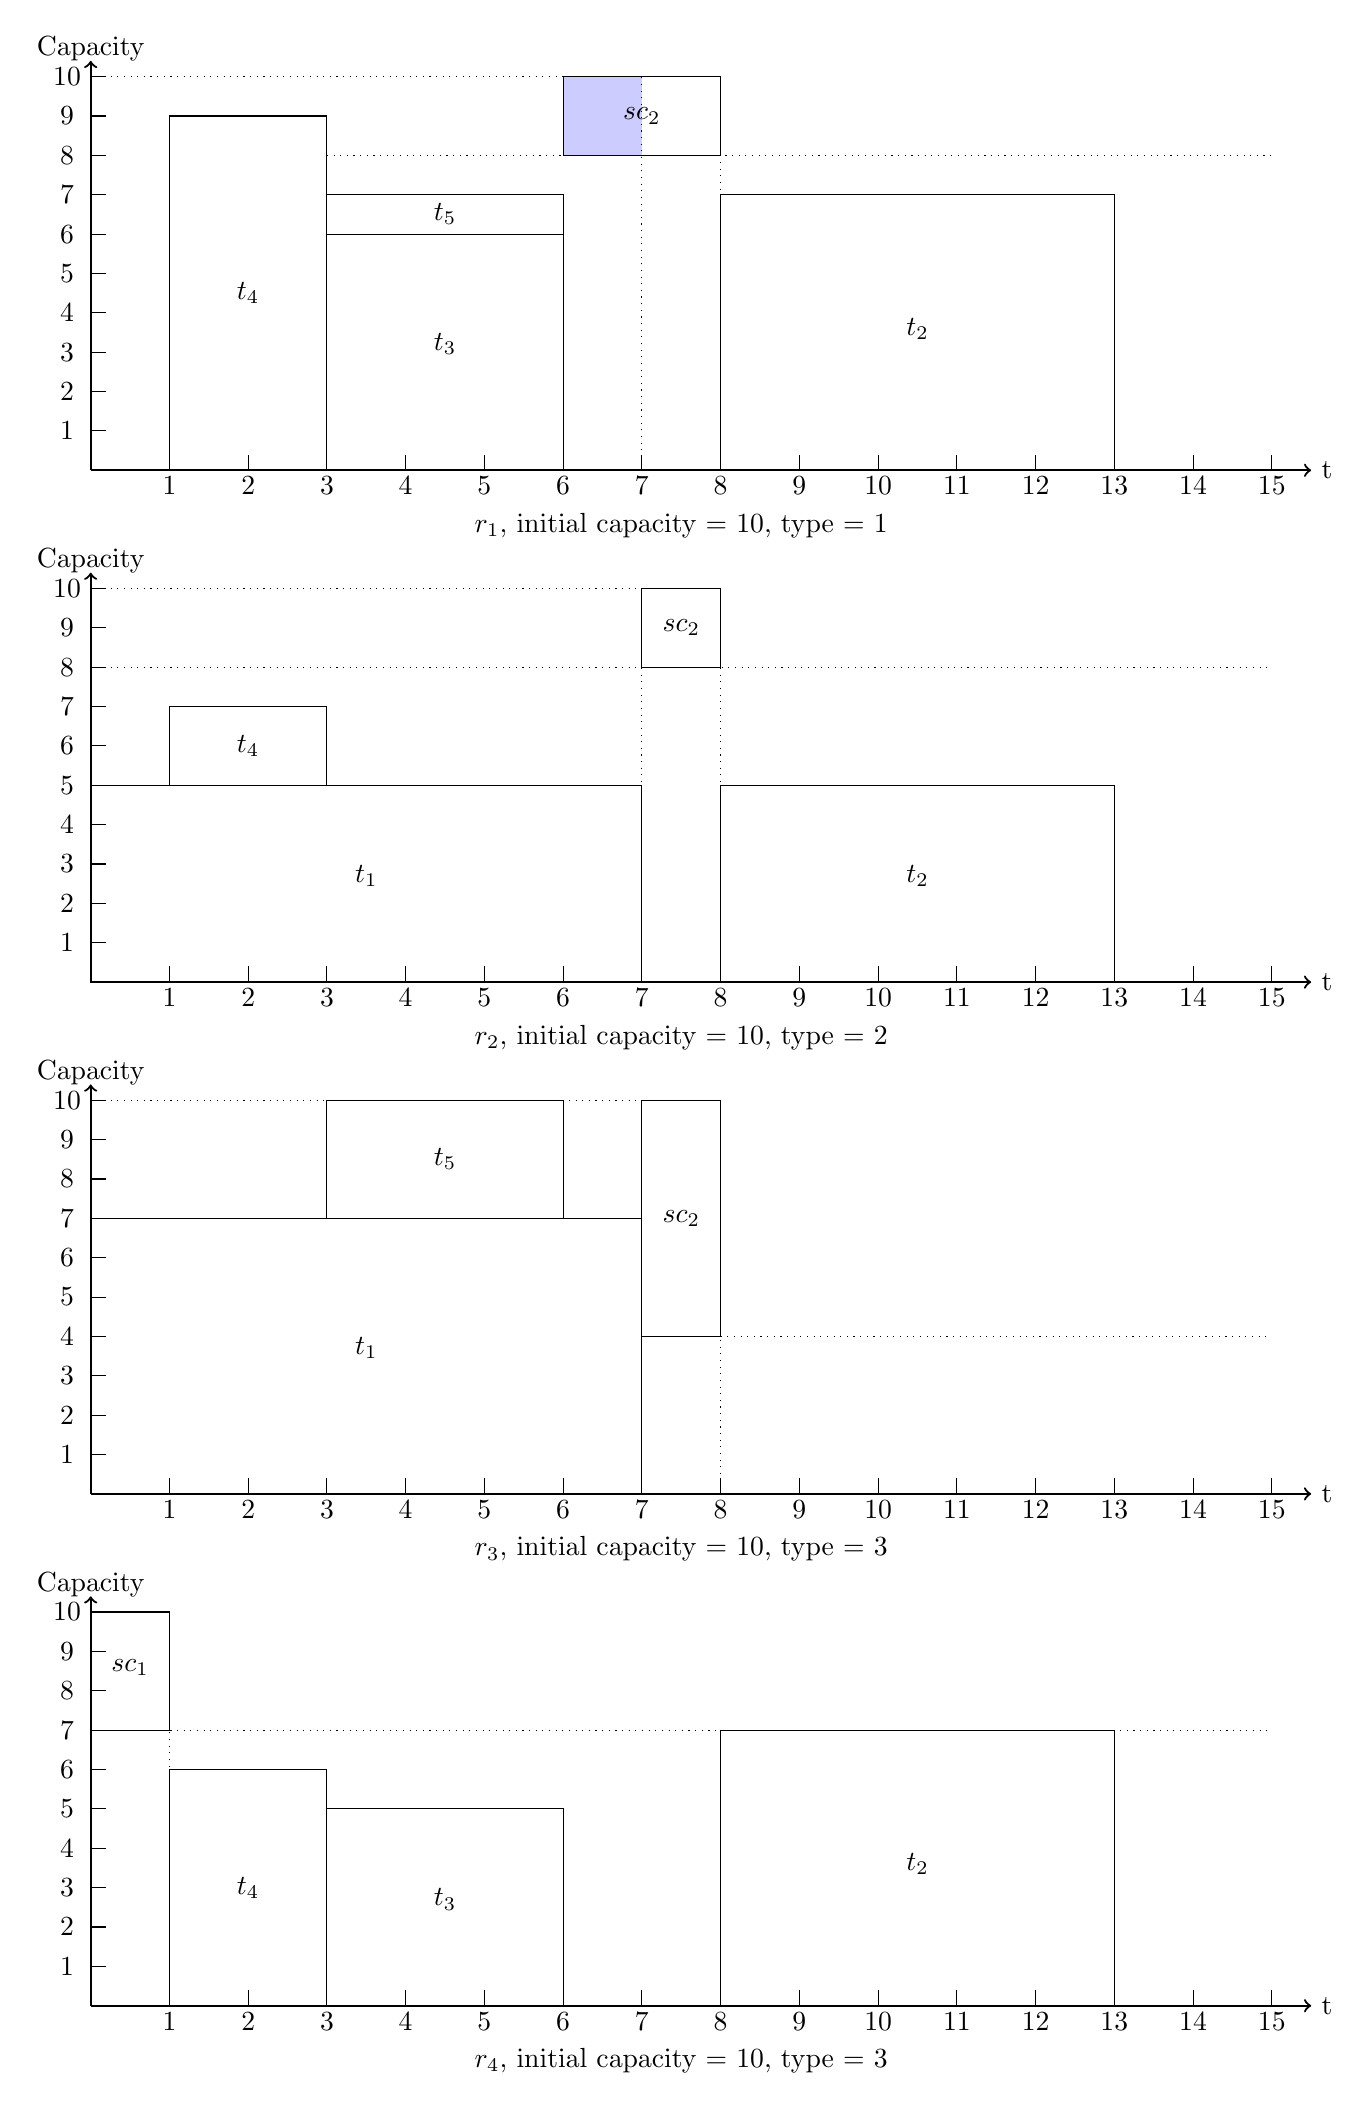
\begin{tikzpicture}
\foreach \x in {0,6.5,13,19.5}
	\draw [->,thick] (15.7cm,\x cm) node{t} (0,\x cm) -- +(15.5cm, 0) ;
\foreach \x in {0,6.5,13,19.5}
	\draw [->,thick] (0,\x cm) -- +(0,5.2 cm);
\foreach \x in {0,6.5,13,19.5}
	\draw[yshift=5.35cm] (0,\x cm) node{Capacity};
\foreach \x in {1,...,15}
	\foreach \y in {0,6.5,13,19.5}
		\draw (\x cm,\y cm) -- +(0,2mm);
\foreach \x in {1,...,15}
	\foreach \y in {0,6.5,13,19.5}
		\draw[yshift=-2mm] (\x cm,\y cm) node{$\x$};
\foreach \y in {0,6.5,13,19.5}
	\foreach \x in {1,...,10}
		\draw[yshift=\y cm] (0,0.5*\x cm) -- +(2mm,0) (-3mm,0.5*\x cm) node{$\x$};

\draw (7.5cm,-7mm) node{$r_4$, initial capacity = 10, type = 3};
\draw[yshift=6.5cm] (7.5cm,-7mm) node{$r_3$, initial capacity = 10, type = 3};
\draw[yshift=13cm] (7.5cm,-7mm) node{$r_2$, initial capacity = 10, type = 2};
\draw[yshift=19.5cm] (7.5cm,-7mm) node{$r_1$, initial capacity = 10, type = 1};

\fill[blue!20!,yshift=19.5cm] (6cm,4cm) rectangle (7cm,5cm);
\draw[yshift=19.5cm] (3cm,0) rectangle (6cm,3cm) (6cm,4cm) rectangle (8cm,5cm) (8cm,0) rectangle (13cm,3.5cm) (1cm,0) rectangle (3cm,4.5cm) (3cm,3cm) rectangle (6cm,3.5cm)  (4.5cm,1.6cm) node{$t_3$} (7cm,4.5cm) node{$sc_2$} (10.5cm,1.8cm) node{$t_2$} (2cm,2.25cm) node{$t_4$} (4.5cm,3.25cm) node{$t_5$};
\draw[dotted,yshift=19.5cm] (0,5cm) -- (7cm,5cm) (3cm,4cm) -- (15cm,4cm) (7cm,0) -- (7cm,5cm) (8cm,4cm) -- (8cm,3.5cm);
\draw[yshift=13cm] (0,0) rectangle (7cm,2.5cm) (7cm,4cm) rectangle (8cm,5cm) (8cm,0) rectangle (13cm,2.5cm) (1cm,2.5cm) rectangle (3cm,3.5cm)  (3.5cm,1.35cm) node{$t_1$} (7.5cm,4.5cm) node{$sc_2$} (10.5cm, 1.35cm) node{$t_2$}  (2cm,3cm) node{$t_4$};
\draw[dotted,yshift=13cm] (0,5cm) -- (7cm,5cm) (0,4cm) -- (15cm,4cm) (7cm,5cm) -- (7cm,0) (8cm,5cm) -- (8cm,0);
\draw[yshift=6.5cm] (0,0) rectangle (7cm,3.5cm) (7cm,2cm) rectangle (8cm,5cm) (3cm,3.5cm) rectangle (6cm,5cm) (3.5cm,1.85cm) node{$t_1$} (7.5cm,3.5cm) node{$sc_2$} (4.5cm,4.25cm) node{$t_5$};
\draw[dotted,yshift=6.5cm] (0,5cm) -- (7cm,5cm) (8cm,2cm) -- (15cm,2cm) (8cm,0) -- (8cm,2cm);
\draw (0,3.5cm) rectangle (1cm,5cm) (3cm,0) rectangle (6cm,2.5cm) (8cm,0) rectangle (13cm,3.5cm) (1cm,0) rectangle (3cm,3cm) (4.5cm, 1.35cm) node {$t_3$} (0.5cm,4.3cm) node{$sc_1$} (10.5cm,1.8cm) node{$t_2$} (2cm,1.5cm) node{$t_4$};
\draw[dotted] (0,3.5cm) -- (15cm,3.5cm) (1cm,0) -- (1cm,3.5cm);
\end{tikzpicture}
}
	\caption{Simple instance schedule chart with 4 resources in 3 different types}
	\label{fig:scheduleChart}
\end{figure}

In every single resource, a schedule is given by a vector of ideal finish times $\bm{f}^{(s)} = \left[f_1^{(s)}, f_2^{(s)},\dots,f^{(s)}_n\right]$,$n=\abs{\mathcal{L}^{(s)}_{k,\tau_0}}$. Even though provider will not schedule $job_\theta\in\mathcal{H}_{k,\tau_0}$, the finish time $f_\theta$ of these job cannot be determined because the waiting in the cooperation. We ignore the type subscript $\alpha$ because all the job assigned here are already type-matched. The schedule model is:

\begin{equation}
\min_{\forall\bm{f}^{(s)}}\left( \max_{\theta\in L^{(s)}}\left\{ f_j^{(s)} - r_\theta - p_\theta \right\} \right) \label{eq:scheduleaim}
\end{equation}
\begin{numcases}{\text{s.t.}}
L^{(s)} = \left\{\theta| job_{\theta}\in \mathcal{L}^{(s)}_{k,\tau_0}\cup\mathcal{H}^{(s)}_{k,\tau_0}\right\} & \label{eq:subscript}\\
f^{(s)}_h \le f_\theta^{(s)} - p_\theta & $h\in\mathcal{P}_\theta$,$\theta\in L^{(s)}$\label{eq:subsequence}\\
G^{(s)} = \left\{\theta | job_{\theta}\in \mathcal{G}_{k,\tau_0}\right\} & \label{eq:activesubscript}\\
f^{(s)}_\theta =  \tau_0 + re_\theta & $\theta\in G^{(s)}$ \label{eq:alreadydefined}\\
\sum_{\theta\in\left\{  \theta' |t_{\theta'} \in\mathcal{G}_{k,\tau}\right\}} q_\theta \le A_{k,\tau}& $\tau \ge \tau_0$ \label{eq:caplimitwithtime} \\
f^{(s)}_\theta \ge \tau_0 + p_\theta & $\theta\in L^{(s)}$ \label{eq:finishconstrain}
\end{numcases}

The schedule aim for each resource \autoref{eq:scheduleaim} is to minimum the maximum delay of jobs. \autoref{eq:subsequence} makes sure that all predecessors of each job finished before the job itself. \autoref{eq:alreadydefined} means that the finish time of activate job is determined. \autoref{eq:caplimitwithtime} makes sure the capacity restriction at every time period and \autoref{eq:finishconstrain} defines the extreme situation of the finish time.
Since \autoref{eq:caplimitwithtime} is a time dependent function, the schedule model cannot be
solved with mixed integer programming (MIP) techniques.

% subsection schedule_the_jobs_in_machine (end)

% \subsection{Tricky problem} % (fold)
% \label{sub:tricky_problems}
% Even though the scheduling procedure exclude the interference of service-call, one tricky problem will occur that it will block some tasks from being processed. Suppose that $t_{i1}$ and $t_{i2}$ both need resource $mr_1$ and $mr_2$, as shown in \autoref{fig:joblock},
% \begin{figure}[htbp]
% 	\centering
% 	\resizebox{.75\textwidth}{!}{% !TEX root = flow_head.tex
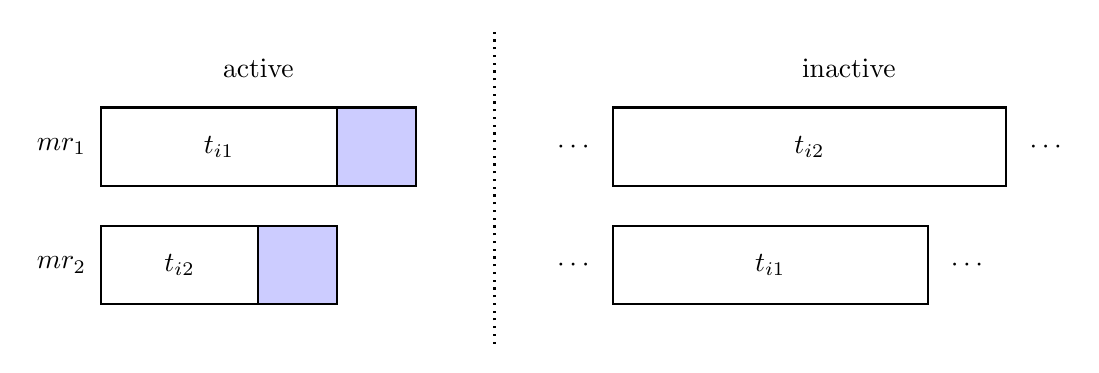
\begin{tikzpicture}

\fill[blue!20!,yshift=1.5cm] (3cm,0) rectangle (4cm,1cm);
\fill[blue!20!] (2cm,0) rectangle (3cm,1cm);
\draw[thick,yshift=1.5cm] (0,0) rectangle (4cm,1cm) (6.5cm,0) rectangle (11.5cm,1cm) (3cm,0) rectangle (4cm,1cm);
\draw[yshift=2cm] (-5mm,0) node{$mr_1$} (1.5cm,0) node{$t_{i1}$} (9cm,0) node{$t_{i2}$} (6cm,0) node{$\cdots$} (12cm,0) node{$\cdots$};
\draw[thick,dotted,xshift=5cm] (0,-5mm) -- (0,3.5cm);
\draw[thick] (0,0) rectangle (3cm,1cm) (6.5cm,0) rectangle (10.5cm,1cm) (2cm,0) rectangle (3cm,1cm);
\draw[yshift=0.5cm] (-5mm,0) node{$mr_2$}  (1cm,0) node{$t_{i2}$} (8.5cm,0) node{$t_{i1}$} (6cm,0) node{$\cdots$} (11cm,0) node{$\cdots$};
\draw[yshift=3cm] (2cm,0) node{active} (9.5cm,0) node{inactive};

\end{tikzpicture}
}
% 	\caption{Simple illustration of job lock problem}
% 	\label{fig:joblock}
% \end{figure}
% $t_{i2}$ is semi-active in $mr_2$ and inactive in $mr_1$, while $t_{i1}$ is semi-active in $mr_1$ and inactive in $mr_2$, however, there is no more space for inactive tasks to stack in, so no matter how long the resource will wait, $t_{i1}$ and $t_i2$ will not be processed and they will block the other tasks from being processed.

% One feasible solution for the job-lock problem is to add the semi-inactive task to the predecessor set of all the other tasks in the same inactive queue list as soon as the status changes.
% subsection tricky_problems (end)
% section design_of_the_ecosystem (end)
